\documentclass{beamer}
\usepackage[italian]{babel}
\usepackage[utf8]{inputenc}
\usepackage{graphicx,hyperref,ru,url}
\usepackage{ragged2e}
\usepackage{pgf}
\usepackage{xcolor}
\usepackage{pifont}
\usepackage{hyperref}
\justifying

% pacchetto per l'inclusione di figure postscript
\usepackage{graphics}

\DeclareGraphicsExtensions{.gif,.png,.pdf,.jpg,.mps}
% pacchetto per inserire figure affiancate
\usepackage{subfigure}
\usepackage[centerlast, bf]{caption}

% The title of the presentation:
%  - first a short version which is visible at the bottom of each slide;
%  - second the full title shown on the title slide;
\title[Prof. Orazio Tomarchio]{\LARGE Facolt\`a di Ingegneria - Universit\`a di Catania}

% Optional: a subtitle to be dispalyed on the title slide
\subtitle{
\Large Smart Intelligent University Communications \\
\Large  Software Engineering Projects\\
}
% The author(s) of the presentation:
%  - again first a short version to be displayed at the bottom;
%  - next the full list of authors, which may include contact information;
\author[Russo, Invincibile, Didomenico]
{\hspace{1.5cm} Relatore         \hspace{5.0cm} Studenti \\
\textbf {Prof. Orazio Tomarchio} \hspace{2.5cm} \textbf{Russo Leandro} \\
\hspace{6.3cm} \textbf{Invincibile Daniele} \\
\hspace{6.2cm} \textbf{Didomenico Nicola} \\
%\vspace{0.5cm}
}

% The institute:
%  - to start the name of the university as displayed on the top of each slide
%    this can be adjusted such that you can also create a Dutch version
%  - next the institute information as displayed on the title slide
\institute[Universit\`a di Catania]{
  Dipartimento di Ingegneria Elettrica, Elettronica e Informatica -- DIEEI \\
  Facolt\`a di Ingegneria Informatica}

% Add a date and possibly the name of the event to the slides
%  - again first a short version to be shown at the bottom of each slide
%  - second the full date and event name for the title slide
\date[27 Febbraio 2015]{27 Febbraio 2015}

\begin{document}

\begin{frame}
  \titlepage
\end{frame}

% Section titles are shown in at the top of the slides with the current section 
% highlighted. Note that the number of sections determines the size of the top 
% bar, and hence the university name and logo. If you do not add any sections 
% they will not be visible.

\section{Problema}
\begin{frame}
  \frametitle{}
   \hyperlink{theorem}
   {\beamergotobutton{Jump to Theorem\#1}
   }
\end{frame}

\section{Iterazione 1}
\begin{frame}[label=theorem]
  \frametitle{}
    \hypersetup{linkbordercolor={0 0.5 0.1}}
    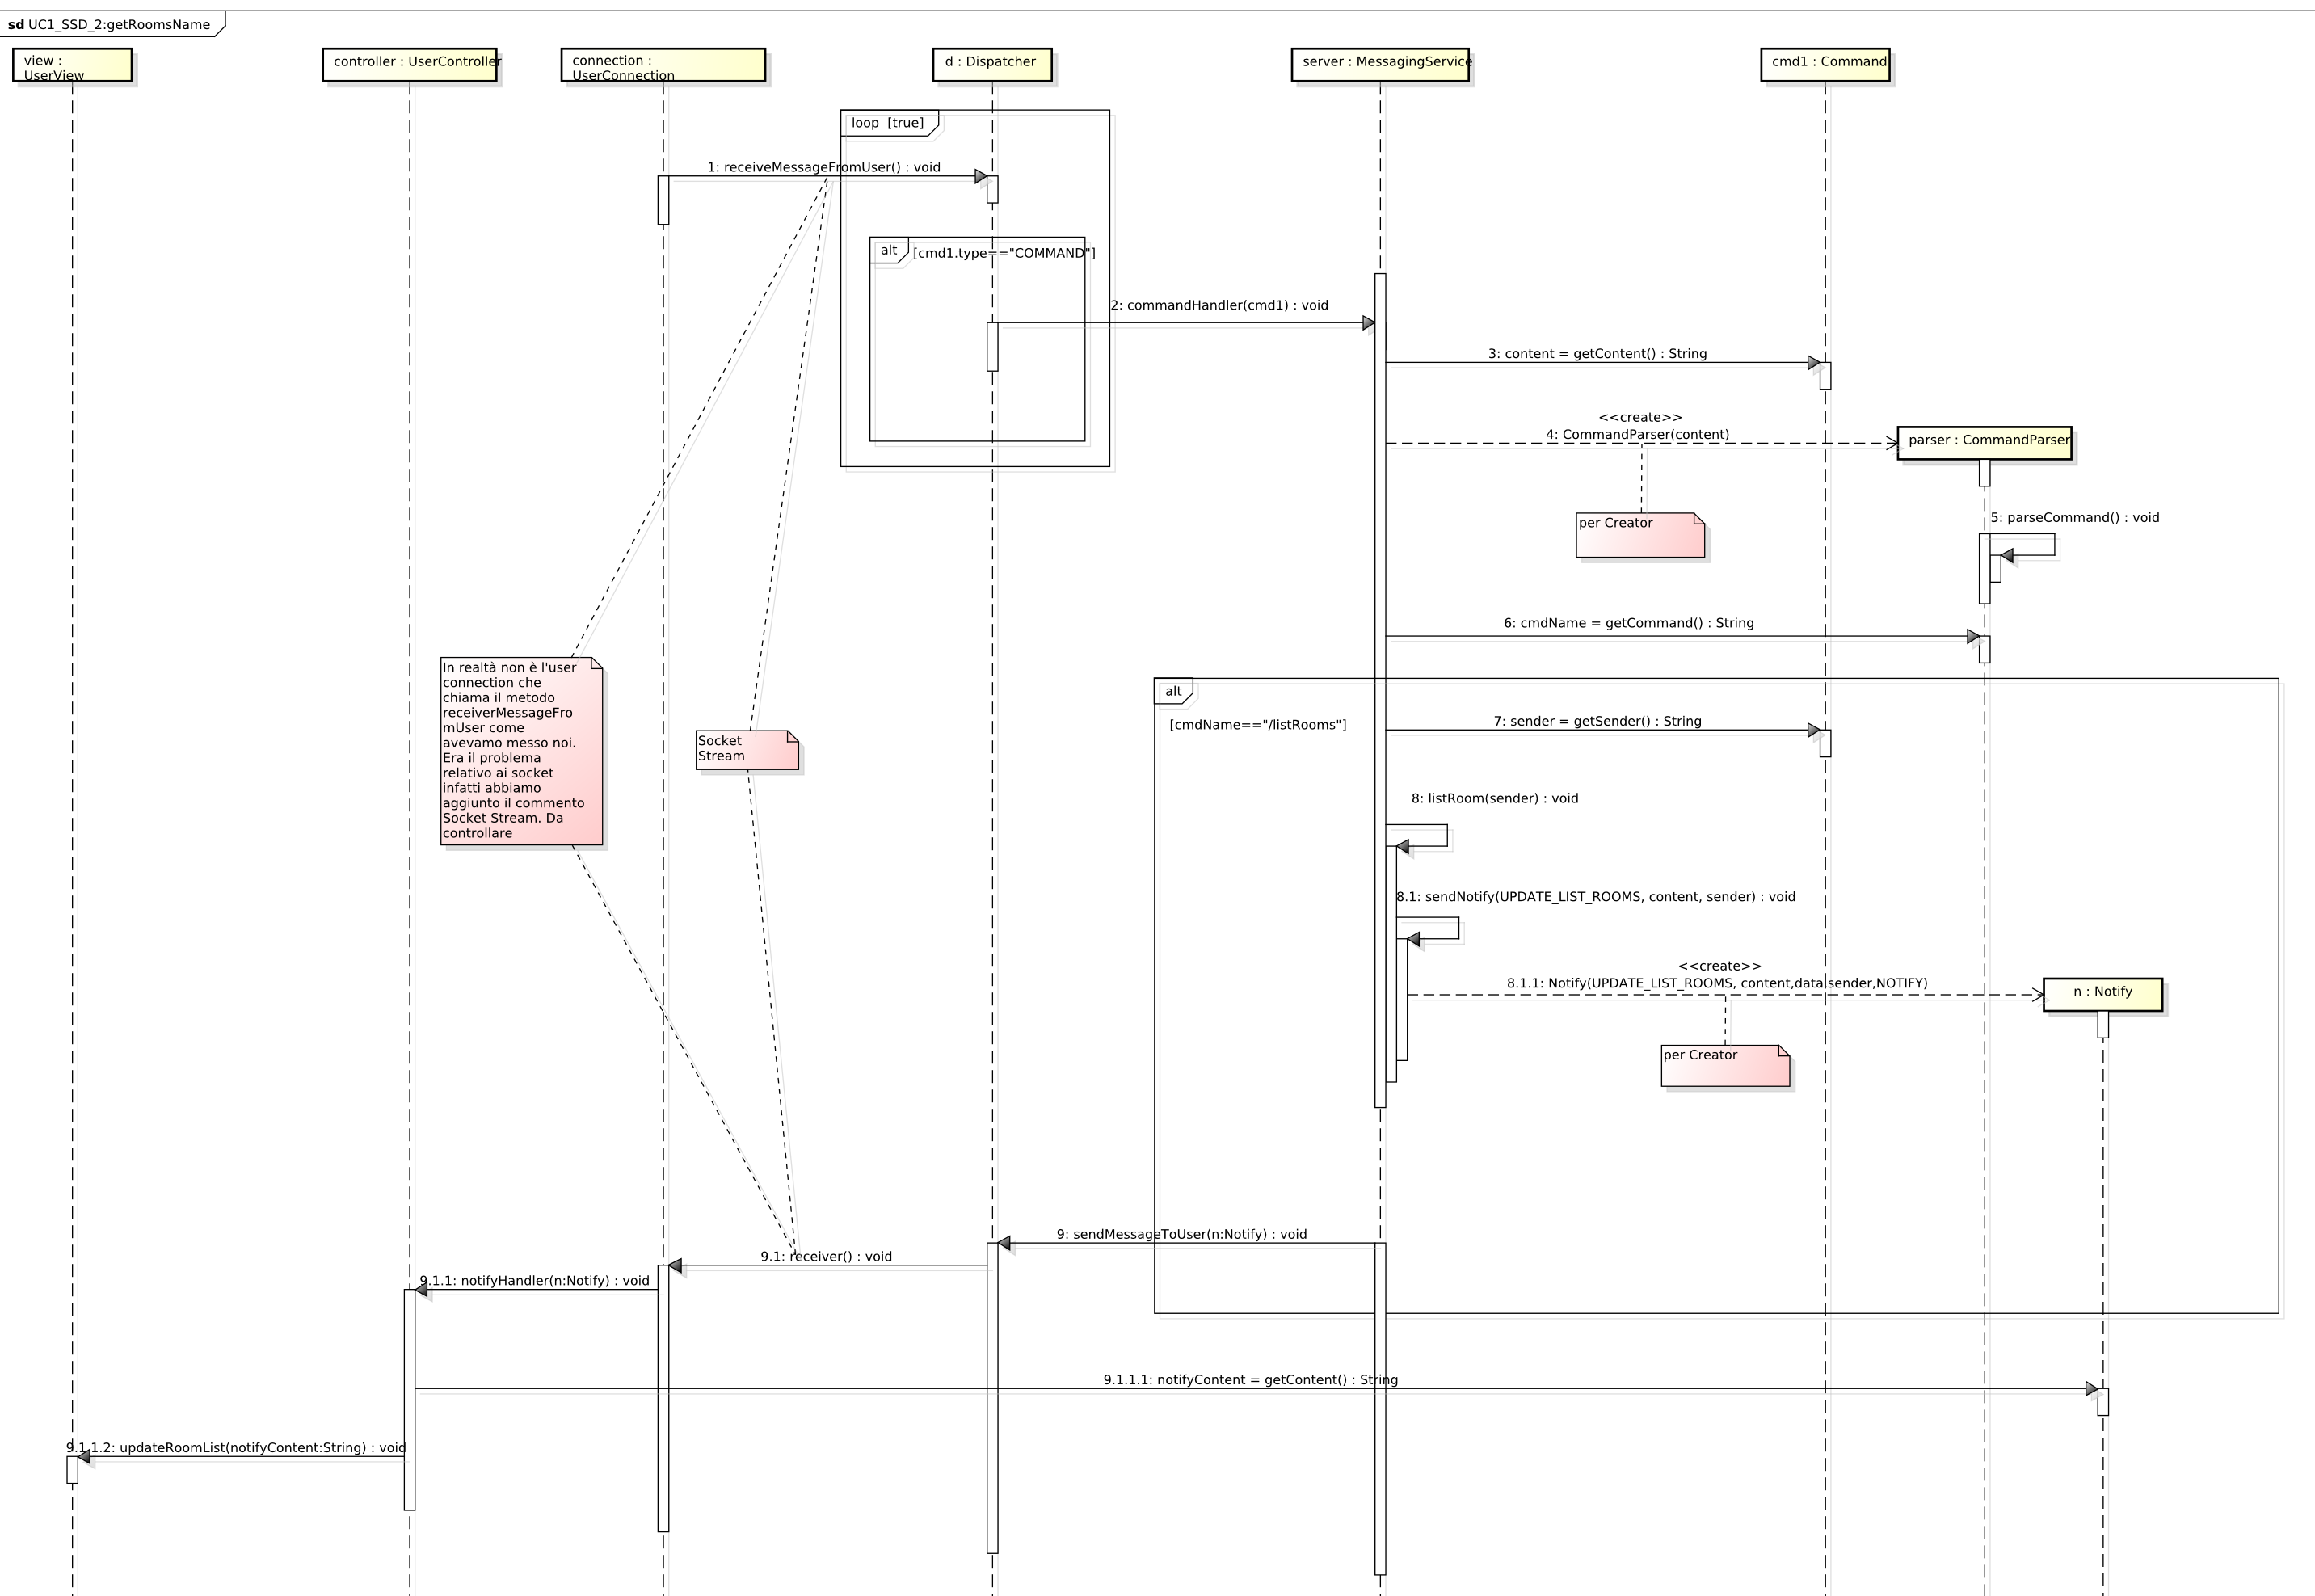
\includegraphics[height=210px, width=305px,]{image/getroomsname.png}{\centering}
    \framezoom <1><2>[border](0 cm,0 cm)(2.5 cm,4.0 cm)
    \framezoom <1><3>[border](5.0 cm,0 cm)(2.5 cm,4.0 cm)
    \framezoom <1><4>[border](0 cm,4 cm)(2.5 cm,3.5 cm)
    \framezoom <1><5>[border](5.0 cm,4 cm)(2.5 cm,3.5 cm)
\end{frame}

\section{Iterazione 1 con Refactoring}
\begin{frame}
  \frametitle{Descrizione delle 5 Fasi ...}
\end{frame}

\section{Iterazione 2}
\begin{frame}
  \frametitle{Descrizione delle 5 Fasi ...}
\end{frame}

\section{Iterazione 3}
\begin{frame}
  \frametitle{Descrizione delle 5 Fasi ...}
\end{frame}


\end{document}
